\section{Results and Analysis}

Our analytics frontend, we first selected Prime Minister Anthony Albanese and examined the weekly average sentiment trend (see Figure \ref{AlbaneseAverageSentiment}). In late March 2025, the Australian federal election was officially called for 3 May, marked by the dashed vertical line in the chart. An interesting pattern appears in the pre-election period. In the weeks leading up to election day, Albanese’s sentiment series shows a temporary improvement: negative sentiment becomes less dominant, while positive sentiment rises and at some points overtakes negative sentiment. Although the chart alone cannot establish a direct causal relationship, it does suggest that the pre-election period was associated with a more favourable online sentiment pattern for Albanese. Notably, Albanese and the Labor government ultimately won re-election, making this shift in sentiment particularly interesting in hindsight.
\begin{figure}[H]	
	\begin{center}
		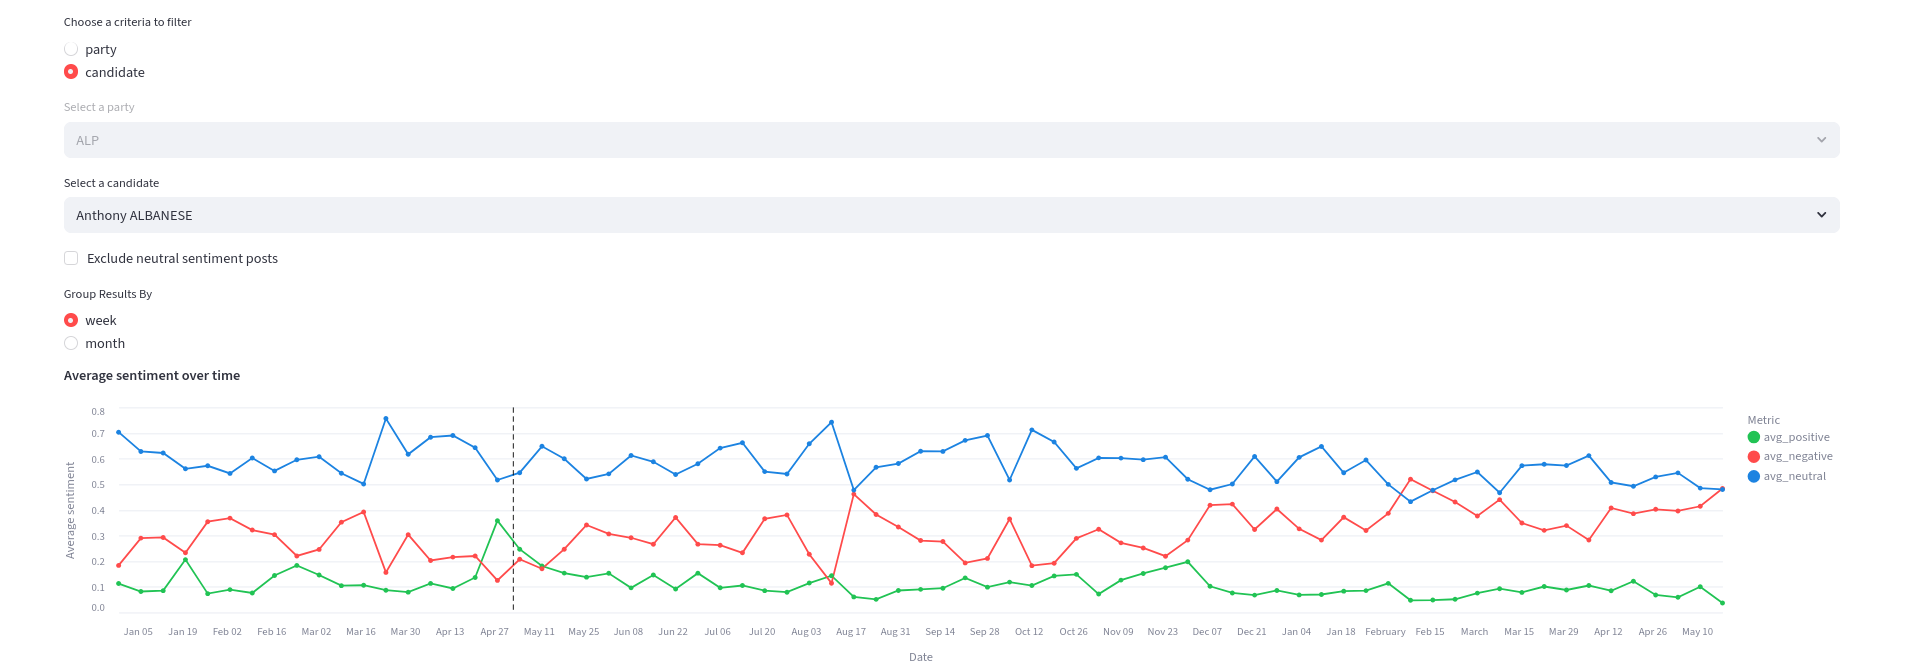
\includegraphics[width=0.75\textwidth]{./assets/AlbaneseAverageSentiment.png}
	\end{center}
	\caption{Weekly Average Sentiment for Anthony Albanese.}
	\label{AlbaneseAverageSentiment}
\end{figure}

A similar pattern can also be observed when we switch the selection from Albanese to his party, the Australian Labor Party (ALP). The ALP chart (Figure \ref{ALPAverageSentiment}) shows a comparable shift over the same period, with positive sentiment strengthening and negative sentiment easing relative to earlier weeks. This parallel movement across both the candidate-level and party-level charts suggests that the change was not limited to Albanese as an individual figure, but was reflected more broadly in Labor’s overall online sentiment during the campaign period. The fact that both Albanese and the ALP later secured victory in the election further reinforces the significance of this shared pre-election sentiment pattern.
\begin{figure}[H]	
	\begin{center}
		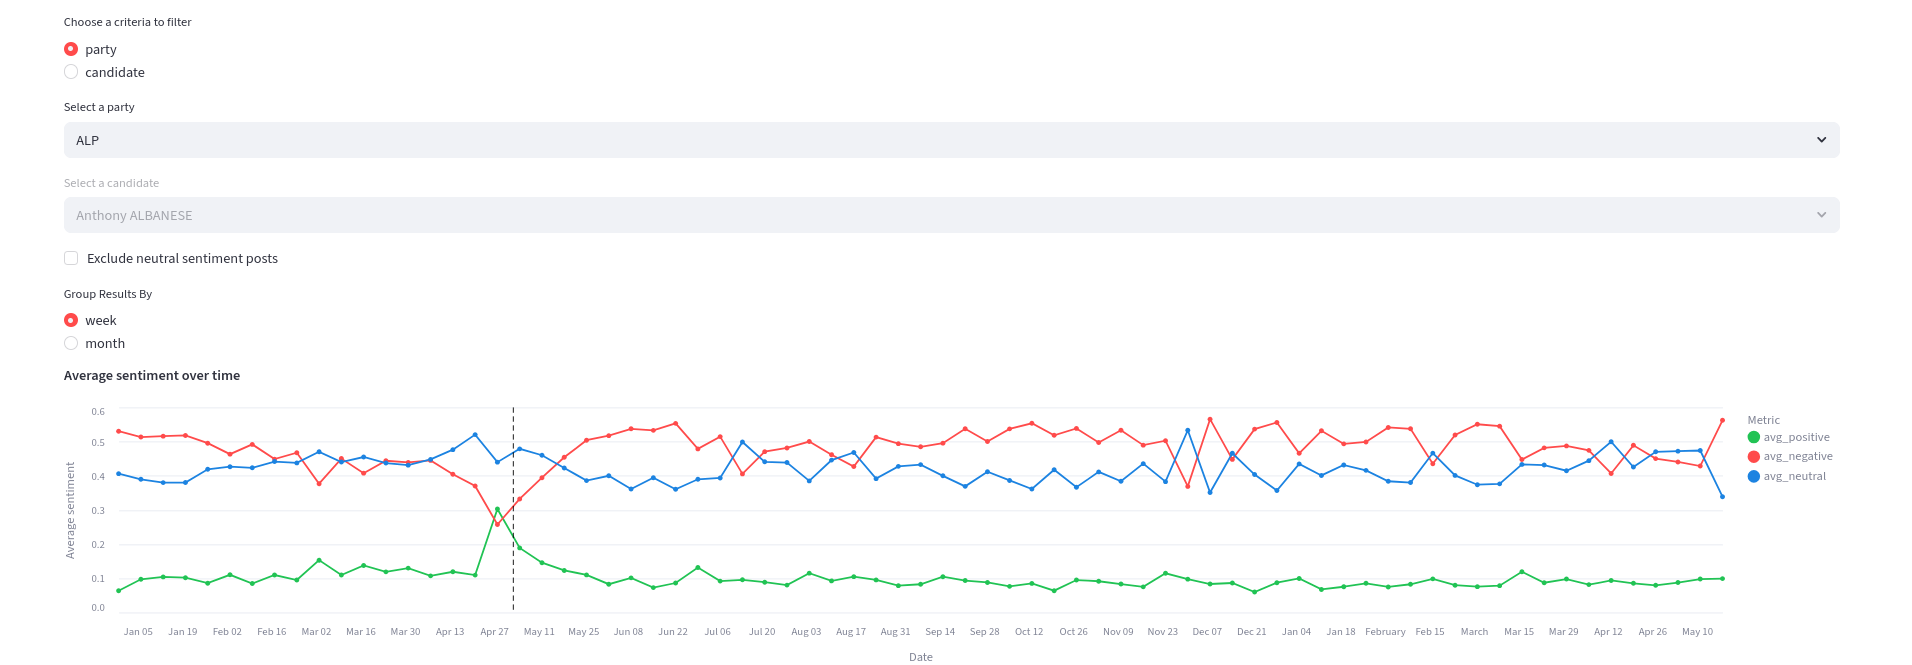
\includegraphics[width=0.75\textwidth]{./assets/ALPAverageSentiment.png}
	\end{center}
	\caption{Weekly Average Sentiment for the Australian Labor Party.}
	\label{ALPAverageSentiment}
\end{figure}

To provide a broader context to these social media trends, we cross-referenced our findings with data harvested from the GDELT project, which tracks global news media sentiment and event locations. When applying the same temporal analysis to the Australian Labor Party's news coverage (Figure \ref{GDELT_ALP_Timeline}) and Anthony Albanese's individual coverage (Figure \ref{GDELT_Albanese_Timeline}), a striking correlation emerges. In both GDELT timelines, the period immediately preceding the May election (marked by the dashed vertical line) shows sentiment peaking towards 0.0 (Factual/Neutral). This confirms that the pre-election "bump" in positive sentiment observed on social media platforms was mirrored by a stabilization and improvement in mainstream media coverage. 

\begin{figure}[H]   
    \begin{center}
        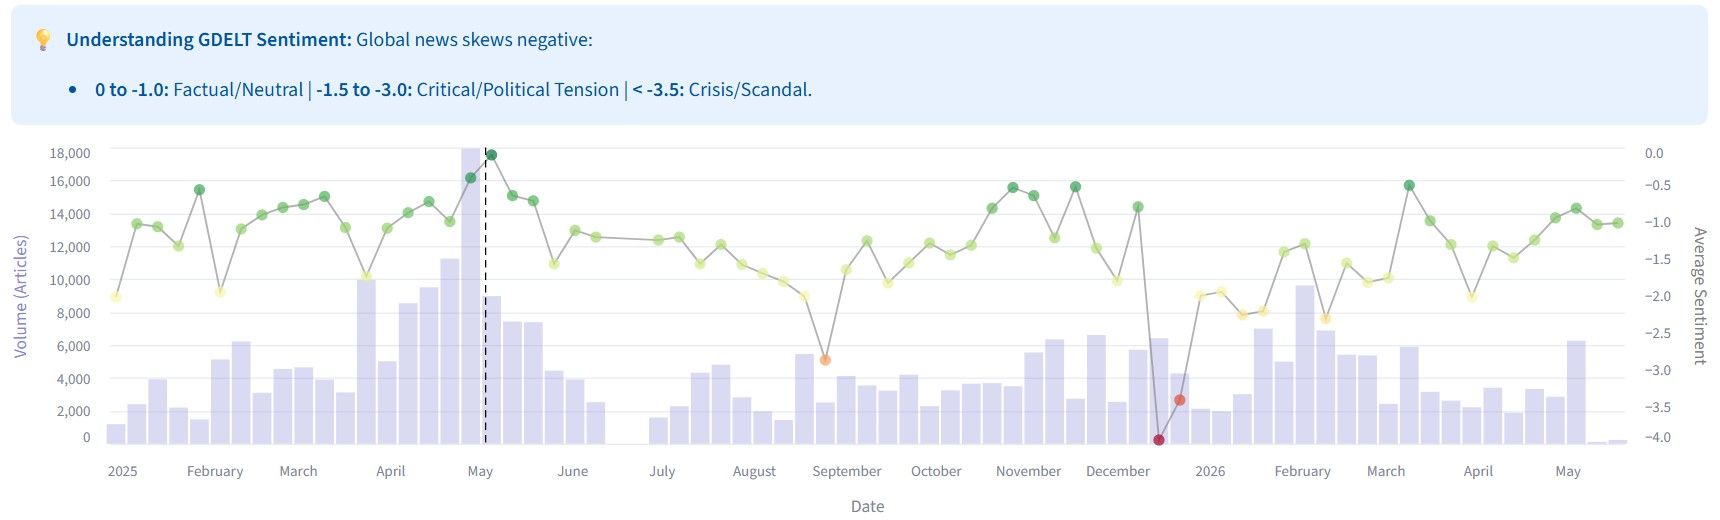
\includegraphics[width=1\textwidth]{./assets/ALP_sentiment_news.jpg}
    \end{center}
    \caption{GDELT Weekly Average Sentiment and Article Volume for the Australian Labor Party.}
    \label{GDELT_ALP_Timeline}
\end{figure}

\begin{figure}[H]   
    \begin{center}
        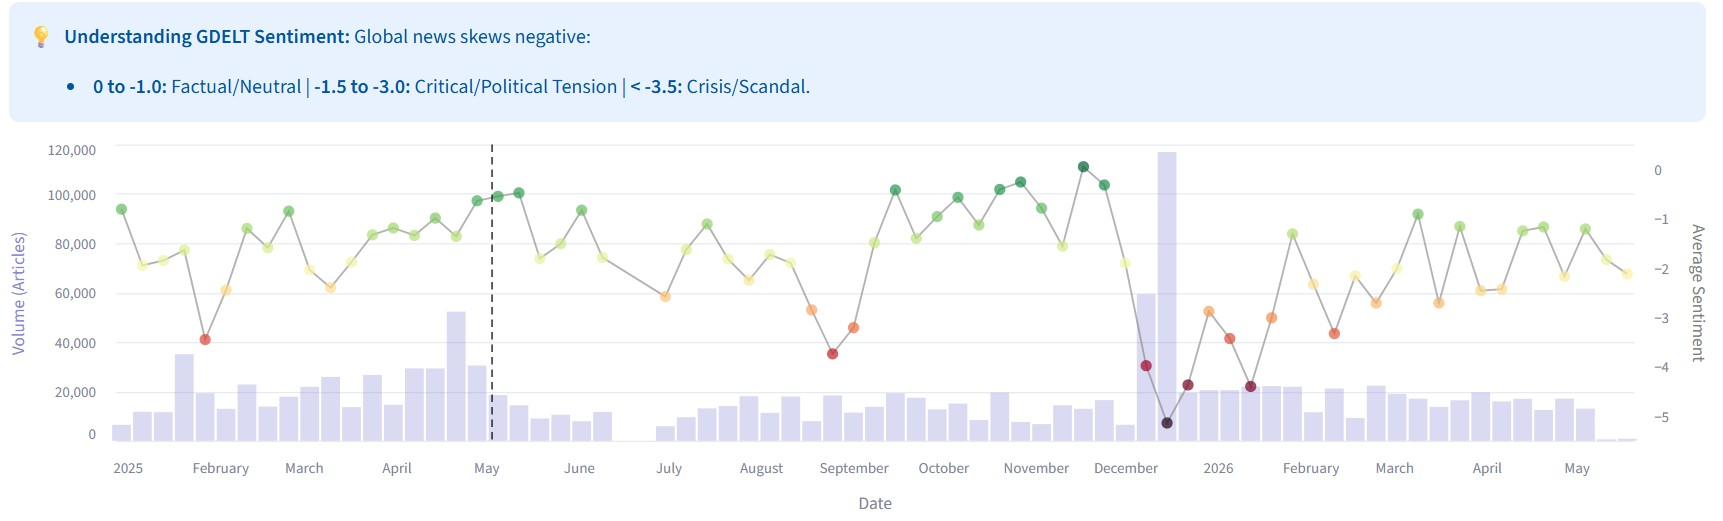
\includegraphics[width=1\textwidth]{./assets/PM_sentiment_news.jpg}
    \end{center}
    \caption{GDELT Weekly Average Sentiment and Article Volume for Anthony Albanese.}
    \label{GDELT_Albanese_Timeline}
\end{figure}

However, mapping the GDELT event data reveals a significant divergence in how the Prime Minister is treated in the media compared to his party, particularly in the post-election landscape. The geographic sentiment map for the Australian Labor Party (Figure \ref{GDELT_ALP_Map}) displays a largely stable, neutral-to-positive distribution (green and yellow nodes) clustered along the eastern seaboard and major metropolitan areas. 

\begin{figure}[H]   
    \begin{center}
        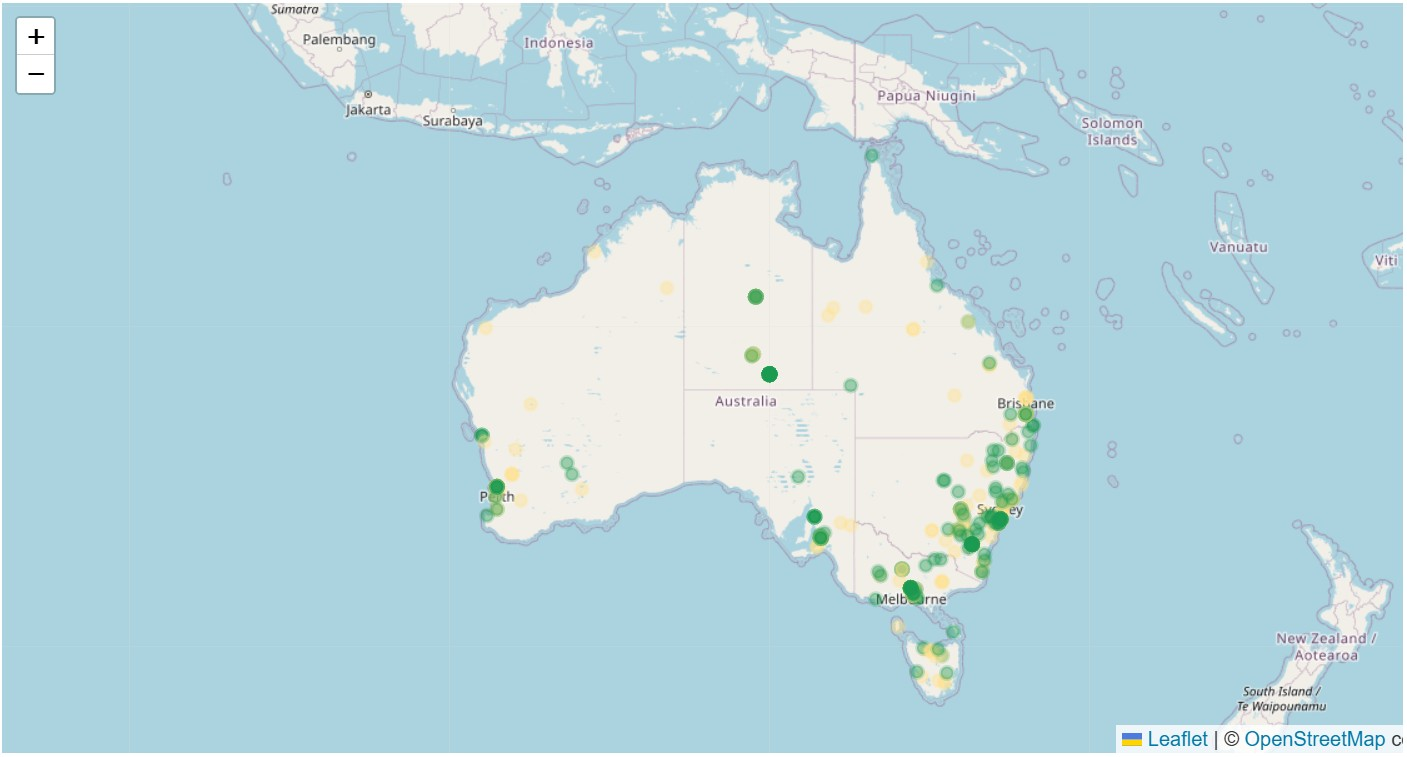
\includegraphics[width=0.85\textwidth]{./assets/Map_ALP.jpg}
    \end{center}
    \caption{GDELT Geographic Sentiment Distribution for the Australian Labor Party.}
    \label{GDELT_ALP_Map}
\end{figure}

Conversely, the geographic map for Anthony Albanese (Figure \ref{GDELT_Albanese_Map}) is distinctly more polarized, featuring highly visible clusters of negative sentiment (red nodes) surrounding major capital cities such as Perth, Melbourne, Sydney, and Brisbane. This geographic polarization aligns with the severe downward spikes into "Crisis/Scandal" territory (sentiment < -3.5) observed in Albanese's timeline during late 2025 and early 2026. This suggests that while social media and news media both reflect a collective party lift during election campaigns, the party leader individually absorbs the vast majority of negative media scrutiny and localized political tension during the actual governance period.

\begin{figure}[H]   
    \begin{center}
        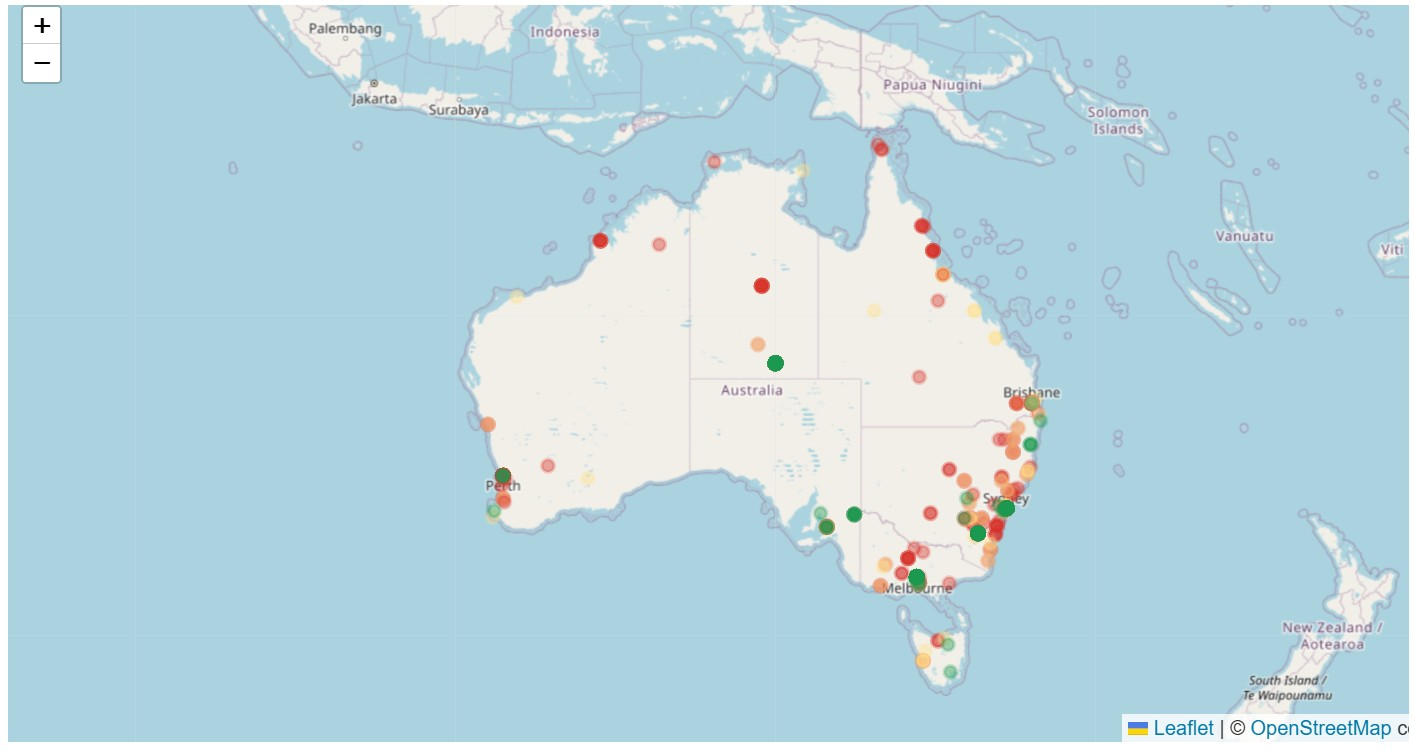
\includegraphics[width=0.85\textwidth]{./assets/Map_PM.jpg}
    \end{center}
    \caption{GDELT Geographic Sentiment Distribution for Anthony Albanese.}
    \label{GDELT_Albanese_Map}
\end{figure}


\section{Conclusion \& Limitations}

This project successfully demonstrated the design, deployment, and operation of a scalable, cloud-native social media analytics platform on the NeCTAR Research Cloud. By leveraging Kubernetes for robust orchestration, Fission for serverless data harvesting, and ElasticSearch for powerful data storage and querying, we established a pipeline capable of ingesting and enriching disparate data streams from BlueSky, Mastodon, YouTube, and the GDELT project.

The architecture’s decoupled nature, facilitated by the Valkey message queue, proved highly effective at absorbing traffic spikes and ensuring fault tolerance during heavy data backfills. Our deployment of ONNX-optimised machine learning models provided critical sentiment and emotion enrichment, proving that complex NLP tasks can be achieved even within strictly resource-constrained, CPU-only academic cloud environments.

However, several limitations remain. Gathering high volumes of strictly relevant, geo-located Australian data proved difficult due to platform API restrictions and the lack of explicit location metadata on modern social networks. Consequently, our reliance on keyword-based filtering required navigating a constant trade-off between precision and recall. Additionally, while our ML pipeline effectively established baseline sentiment trends, it struggles with the nuances of sarcasm, irony, and Australian colloquialisms. Finally, due to absolute hardware limits on our NeCTAR cluster, some components—such as our ML inference pod—operate as single points of failure, preventing true high availability.

Despite these limitations, the system successfully meets the core objectives of the assignment. It provides a flexible, dynamically scalable framework that researchers can use to capture the essence of public discourse and visualize shifting political attitudes via interactive Jupyter Notebook analytics. Future work could improve upon this foundation by fine-tuning the NLP models for Australian political slang and migrating the database into a fully replicated, multi-node cluster to ensure complete fault tolerance.

\subsection*{Declaration of Generative AI Usage}
During the preparation of this project, the team utilised Generative AI (Google Gemini Flash \& Pro 3.1 and Claude Sonnet 4.6) to assist with proofreading, structuring the LaTeX report, and refining academic language. These specific models were selected due to their strong proficiency in processing complex technical context and producing highly structured, academic prose. All system architecture, code, analytical scenarios, and all concepts represent the original work of the student team.
